
\noindent \textbf{3. mac338-2011, p2} Você conhece a tartaruga Yertle?

O trono de Yertle é composto de uma pilha de tartarugas, conforme a figura \ref{fig:6.23-1}.

\begin{center}
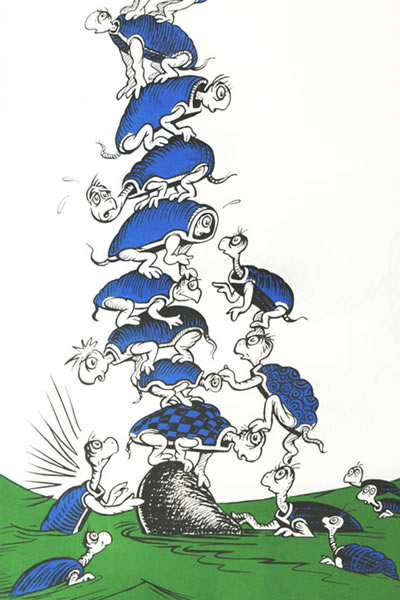
\includegraphics[width=0.45\textwidth]{q6-23}
\label{fig:6.23-1}
\end{center}

Cada tartaruga, ao se alistar para fazer parte do trono, fornece o seu peso e a sua força. A sua missão é determinar uma pilha de tartarugas, dentre as alistadas, o maior possível, em que nenhuma tartaruga quebre por entrar na pilha. O peso de cada tartaruga é dado em gramas, e a sua força é em gramas também.

A força de uma tartaruga indica quanto peso, incluindo o seu, ela aguenta. Ou seja, uma tartaruga de peso 300 gramas que tem força de 1000 gramas pode carregar 700 gramas de tartarugas sobre ela. Numa pilha válida de tartarugas, cada tartaruga tem força para sustentar as tartarugas que estão acima dela na pilha. Considere as três possíveis maneiras de ordenarmos as tartarugas:\\[6pt]

\noindent (i) em ordem decrescente de peso;\\[2pt]
(ii) em ordem decrescente de força;\\[2pt]
(iii) em ordem decrescente de força menos peso.\\[6pt]

\noindent (a) Para cada uma destas três ordens, prove ou dê um contra-exemplo para a seguinte afirmação: qualquer pilha válida de tartarugas pode ser reorganizada para que as tartarugas apareçam nesta ordem, de baixo para cima, e a pilha continue válida. Dica: a afirmação é verdadeira para apenas uma das ordens.\\[2pt]
\noindent (b) Seja n o número de tartarugas, $p[1..n]$ o peso das $n$ tartarugas e $f[1..n]$ a força das $n$ tartarugas.

Suponha que as tartarugas estão ordenadas na ordem correta (a que funciona das três acima) e que todas tem peso maior que zero. Seja $c[i, w]$ o número de tartarugas na maior pilha válida de tartarugas composta de tartarugas de 1 a $i$ com peso igual a $w$. (Se não houver pilha válida, deixe $c[i,w] = -1$.)

Escreva uma recorrência válida para $c[i, x]$ (acho que é w aqui). Não esqueça de definir o caso base da recorrência! Explique porque sua recorrência está correta, ou seja, prove (indutivamente) que $c[i,w]$ é o número de tartarugas na maior pilha válida de tartarugas composta de tartarugas de 1 a $i$ com peso igual a $w$.\\[2pt]
\noindent (c) A partir da sua recorrência, escreva (em pseudo-código, como nas aulas) um algoritmo de programação
dinâmica que, dados $n$, $p$ e $f$, representando os dados de $n$ tartarugas, determine e devolva o número de tartarugas em uma pilha válida máxima formada com estas tartarugas. O seu algoritmo deve claramente corresponder à sua recorrência.\\[2pt]
\noindent (d) Analise o consumo de tempo do seu algoritmo em função de $n$.